\documentclass[conference]{IEEEtran}
\IEEEoverridecommandlockouts
% The preceding line is only needed to identify funding in the first footnote. If that is unneeded, please comment it out.
%Template version as of 6/27/2024

\usepackage{cite}
\usepackage{amsmath,amssymb,amsfonts}
\usepackage{algorithmic}
\usepackage{graphicx}
\usepackage{textcomp}
\usepackage{xcolor}
\def\BibTeX{{\rm B\kern-.05em{\sc i\kern-.025em b}\kern-.08em
    T\kern-.1667em\lower.7ex\hbox{E}\kern-.125emX}}
%
%
% Sepetmber 23, 2024
\usepackage{cleveref}
%

%
%
% September 23, 2024
\usepackage{enumitem}
%

\begin{document}

\title{Accessible Legislative Information: Automatic Summarisation of Zambian Legislative Documents}

\author{\IEEEauthorblockN{1\textsuperscript{st} FName1 LName1}
\IEEEauthorblockA{\textit{dept. name of organization (of Aff.)} \\
\textit{name of organization (of Aff.)}\\
City, Country \\
fname1.lname1@institution.xx}
\and
\IEEEauthorblockN{2\textsuperscript{nd} FName2 LName2}
\IEEEauthorblockA{\textit{dept. name of organization (of Aff.)} \\
\textit{name of organization (of Aff.)}\\
City, Country \\
fname2.lname2@institution.xx}
\and
\IEEEauthorblockN{3\textsuperscript{rd} FName3 LName3}
\IEEEauthorblockA{\textit{dept. name of organization (of Aff.)} \\
\textit{name of organization (of Aff.)}\\
City, Country \\
fname3.lname3@institution.xx}
\and
\IEEEauthorblockN{4\textsuperscript{th} FName4 LName4}
\IEEEauthorblockA{\textit{dept. name of organization (of Aff.)} \\
\textit{name of organization (of Aff.)}\\
City, Country \\
fname4.lname4@institution.xx}
\and
\IEEEauthorblockN{5\textsuperscript{th} FName5 LName5}
\IEEEauthorblockA{\textit{dept. name of organization (of Aff.)} \\
\textit{name of organization (of Aff.)}\\
City, Country \\
fname5.lname5@institution.xx}
}

\maketitle

\begin{abstract}
The National Assembly of Zambia produces a number of important legislative documents which are publicly accessible via its Website. One of the documents published by the National Assembly of Zambia are Bills and Acts, which all form the Laws of Zambia. The Acts and Bills are ideally meants to be open and accessible to the general citizenery, however, prior studies conducted have highlighted the lack of ease of access and difficulties with interpretation of such documents and the two main barriers to enabling open and accessible legal information. This paper presents a potentially viable solution to addressing the chellenges with facilitating open and accessible legislative documents by leveraging the use of Natural Language Processing techniques for automatically summarising legislative documents. Specifically, the study was aimed at examinting barriers faced by individuals when comprehending legislative documents and, additionally, determining the feasibility of implementing NLP modules capable of generating concise summaries of legislative documents. In order to understand challenges faced when comprehending legal documents, 150 undergraduate students were sampled from the University of Zambia using random sampling. To determine the feasibility of using NLP techniques to provide concise summaries of legislative documents, two (2) NLP models—an abstractive summarisation model and extractive summarisation model. A human evaluation strategy was used to perform a comparative evaluation of the two (2) NLP models, in order to determine the more effective approach. A significant portion—approximately 74.29\%—of participants reported 'Never' (33.99\%) or 'Rarely' (40.3\%) engaging with legislative documents. In contrast, (25.71\%) indicated frequent or very frequent interaction. This distribution underscores a significant gap in familiarity and engagement with Zambian legislative materials among the study participants. In assessing participants' overall understanding of legal documents, the majority (43.5\%) expressed a neutral perception, suggesting that they found these documents neither easy nor hard to understand. The majority of the human evaluators had a preference for the abstractive summarisation model, indicating that its brevity, simplicity, and directness as reasons for their choice. In addition, the results of the abstractive summarisation model were stated as being easier to understand.
\end{abstract}

\begin{IEEEkeywords}
document summarisation, legislative documents, natural language processing, zambia.
\end{IEEEkeywords}

\section{Introduction}
\label{sec:introduction}
The National Assembly of Zambia is mandated by law to “To execute the legislative, oversight, representative and budgetary functions for enhanced democratic governance” \cite{NationalAssembly2023Objectives}. In the 2022-2026 strategic plan \cite{NationalAssembly2021Strategic}, the “Strategic Objective 2.2” aims to “Enhance Public Perceptions of the National Assembly” by making parliament open and accessible to the public and, additionally strengthening ICT platforms for public engagement.

While parliament, and entities such as the Zambia Legal Information Institute (ZambiaLII) \cite{ZambiaLII2024Website}, publicly makes available important legislation, interpretation of the documents is problematic due to the size of the documents and the vocabulary used. Masson and Tahir report that the barriers associated with providing open and accessible legal information relies on two factors: ease of access and the capacity to interpret the documents \cite{Masson2016Legal}.

This paper is organised as follows: \Cref{sec:introduction} provides context and background information associated with the studies conducted; \Cref{sec:related_work} comprehensively discusses existing work; \Cref{sec:methodology} outlines the methodological approaches employed when conducting the studies; \Cref{sec:results_and_discussion} discusses the findings and, finally, \Cref{sec:conclusion} outlines concluding remarks and potential future work.

\section{Related Work}
\label{sec:related_work}
Xxxxx xxxxx xxxxx  xxxxx  xxxxx  xxxxx  xxxxx  xxxxx  xxxxx  xxxxx  xxxxx  xxxxx  xxxxx  xxxxx  xxxxx  xxxxx  xxxxx  xxxxx  xxxxx  xxxxx  xxxxx  xxxxx  xxxxx  xxxxx  xxxxx  xxxxx  xxxxx  xxxxx  xxxxx  xxxxx  xxxxx  xxxxx  xxxxx  xxxxx  xxxxx  xxxxx  xxxxx  xxxxx  xxxxx  xxxxx  xxxxx  xxxxx  xxxxx  xxxxx  xxxxx  xxxxx  xxxxx  xxxxx  xxxxx  xxxxx  xxxxx  xxxxx  xxxxx  xxxxx  xxxxx  xxxxx  xxxxx  xxxxx  xxxxx  xxxxx  xxxxx  xxxxx  xxxxx  xxxxx  xxxxx  xxxxx  xxxxx  xxxxx  xxxxx  xxxxx  xxxxx  xxxxx  xxxxx  xxxxx  xxxxx.

\section{Methodology}
\label{sec:methodology}
A mix-methods approach was employed to conduct the studies outlined in this paper as follows:
\begin{itemize}
    \item A survey, outlined in \Cref{sec:methodology:understanding_legislation_documents} was conducted with students at University X
    \item NLP summarisation models were implemented as outlined in \Cref{sec:methodology:summarisation_models_implementaiton}
    \item A controlled comparative evaluation was performed with human evaluators, as outlined in \Cref{sec:methodology:summarisation_models_analysis}, in order to determine the perceived effective summarisation technique
\end{itemize}

\subsection{Understanding Legislative Documents}
\label{sec:methodology:understanding_legislation_documents}
In order to understand participants' with legislative documents and, additionally, challenges associated with comprehending legislative documents, a survey was conducted with randomly sampled full-time undergraduate students at The University of Zambia. Socialdemographic factors---gender, age, school/faculty, programme of study and year of study---were collected from participants, in addition frequency with which legislative documents were accessed and, finally, difficulties with comphrehending legislative documents using "Statutory Instrument No. 12 of 2018"---shown in \Cref{fig:methodology:understanding_legislation_documents:si18_2018}---as a reference.

\begin{figure*}%%%%%[htbp]
\fbox{%
\scalebox{0.315}{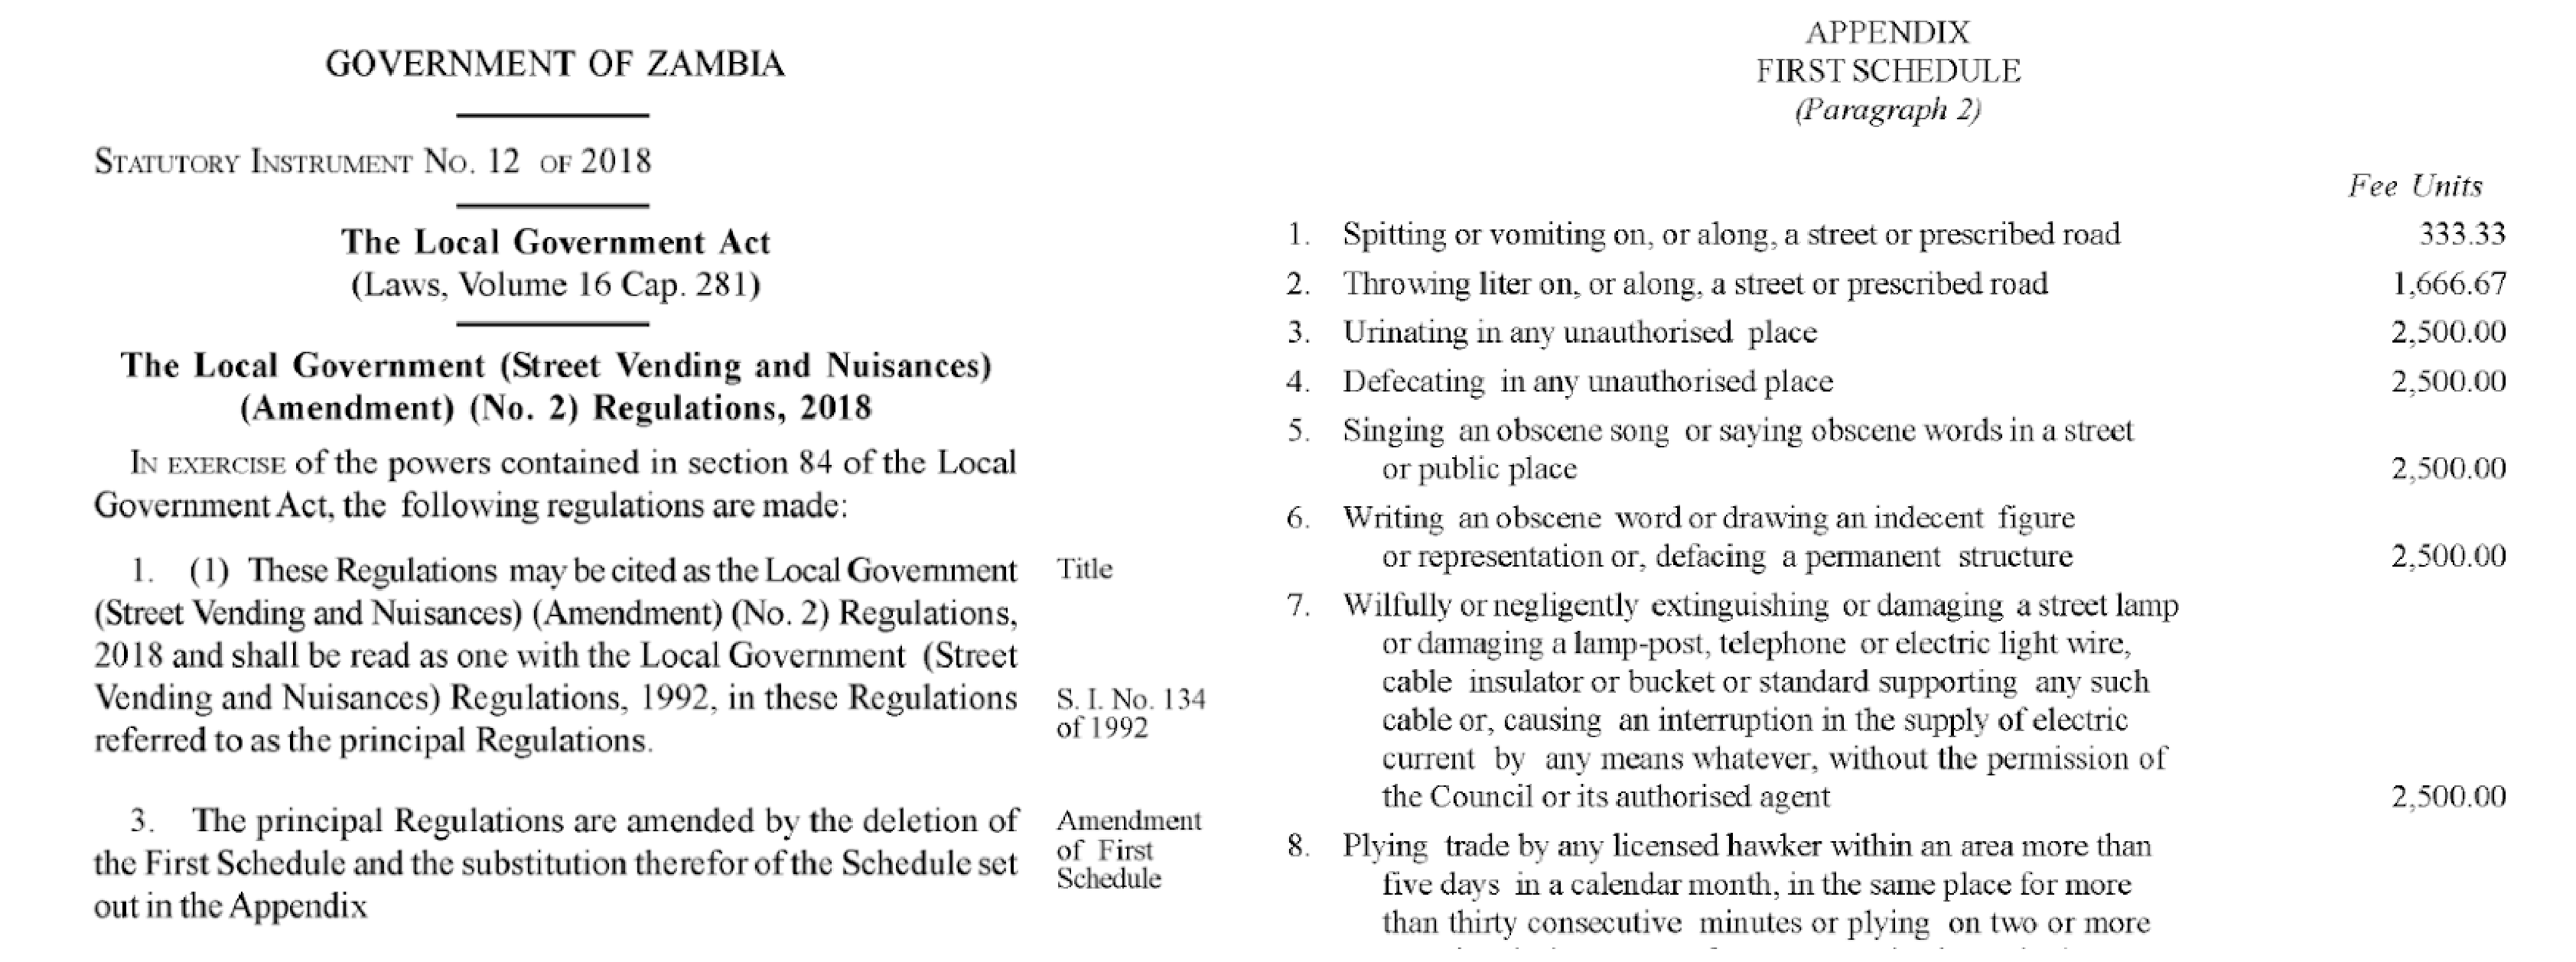
\includegraphics{figures/img-icict24-statutory_instrument12_2018.eps}}
}%
\caption{Statutory Instrument 18 of 2018: Street Vending and Nuisances.}
\label{fig:methodology:understanding_legislation_documents:si18_2018}
\end{figure*}

\subsection{Summarisation Models: Design and Implementation}
\label{sec:methodology:summarisation_models_implementaiton}
The implementation of the NLP summarisation models and pipelines was guided by the Cross-industry Standard Process for Data Mining (CRISP-DM) model \cite{Wirth2000CRISPDM}, with the six (6) phases used as follows:
\begin{enumerate}[label=\textbf{Phase \arabic*.}, leftmargin=*]
    \item Business Understanding---Acts and Bills available on the National Assembly of Zambia Website were analysed to understand the structure of legislative documents
    \item Data Understanding---Data sources were identified, with data extraction conducted on publicly available PDF documents
    \item Data Preparation---Data was pre-processed using common text pre-processing techniques
    \item Modelling---NLP models were implemented in order to summarise legislative documents
    \item Evaluation---Human evaluators were used to determine the most effective summarisation technique---abstractive and extractive summarisation
    \item Deployment---A simple Web-based interface was implemented to comparatively evaluate the two abstractive and extractive summarisations models.
\end{enumerate}

In order to implement effective NLP summarisation models, focus group discussions were held with University of Zambia Law students, in order to understand elements that comprise legislative documents.

Two NLP summarisation models were implemented use two common summarisation techniques: abstractive summarisation and extractive summarisation.

\subsection{Summarisation Models: Comparative Analysis}
\label{sec:methodology:summarisation_models_analysis}
In order to comparatively evaluate the abstractive and extractive summarisation models, a controlled experiment was conducted with human evaluators.

\subsubsection{Task Design}
\label{sec:methodology:summarisation_models_analysis:task_design}
The National Pension Scheme Act No. 1 of 2023\footnote{https://www.parliament.gov.zm/node/11020} was used as input to the two summarisation models and corresponding summaries generated.

\subsubsection{Experimental Design}
\label{sec:methodology:summarisation_models_analysis:experimental_design}
A comparative analysis between the abstractive summarisation model and extractive summarisation model was performed. The study was conducted using a within-subject design, with counterbalancing applied by altering the summarisation models they initially read and rated.

\subsubsection{Procedure}
\label{sec:methodology:summarisation_models_analysis:procedure}
Each participant was required to sign a consent form and subsequently required to read the "National Pension Scheme Act No. 1 of 2023" document and, additionally, the two corresponding summaries. Finally, participants were required to complete a questionnaire design to evaluate the following:
\begin{itemize}
    \item Relevance of each of the two summaries, relative to the original document
    \item Readability ofeach of the two summaries
    \item Prefered summary, when comparing the two generated summaries
\end{itemize}

\section{Results and Discussion}
\label{sec:results_and_discussion}
Xxxxx xxxxx xxxxx  xxxxx  xxxxx  xxxxx  xxxxx  xxxxx  xxxxx  xxxxx  xxxxx  xxxxx  xxxxx  xxxxx  xxxxx  xxxxx  xxxxx  xxxxx  xxxxx  xxxxx  xxxxx  xxxxx  xxxxx  xxxxx  xxxxx  xxxxx  xxxxx  xxxxx  xxxxx  xxxxx  xxxxx  xxxxx  xxxxx  xxxxx  xxxxx  xxxxx  xxxxx  xxxxx  xxxxx  xxxxx  xxxxx  xxxxx  xxxxx  xxxxx  xxxxx  xxxxx  xxxxx  xxxxx  xxxxx  xxxxx  xxxxx  xxxxx  xxxxx  xxxxx  xxxxx  xxxxx  xxxxx  xxxxx  xxxxx  xxxxx  xxxxx  xxxxx  xxxxx  xxxxx  xxxxx  xxxxx  xxxxx  xxxxx  xxxxx  xxxxx  xxxxx  xxxxx  xxxxx  xxxxx  xxxxx.

\section{Conclusions and Future Work}
\label{sec:conclusion}
Xxxxx xxxxx xxxxx  xxxxx  xxxxx  xxxxx  xxxxx  xxxxx  xxxxx  xxxxx  xxxxx  xxxxx  xxxxx  xxxxx  xxxxx  xxxxx  xxxxx  xxxxx  xxxxx  xxxxx  xxxxx  xxxxx  xxxxx  xxxxx  xxxxx  xxxxx  xxxxx  xxxxx  xxxxx  xxxxx  xxxxx  xxxxx  xxxxx  xxxxx  xxxxx  xxxxx  xxxxx  xxxxx  xxxxx  xxxxx  xxxxx  xxxxx  xxxxx  xxxxx  xxxxx  xxxxx  xxxxx  xxxxx  xxxxx  xxxxx  xxxxx  xxxxx  xxxxx  xxxxx  xxxxx  xxxxx  xxxxx  xxxxx  xxxxx  xxxxx  xxxxx  xxxxx  xxxxx  xxxxx  xxxxx  xxxxx  xxxxx  xxxxx  xxxxx  xxxxx  xxxxx  xxxxx  xxxxx  xxxxx  xxxxx.


% % % % % \section*{References}

\bibliographystyle{IEEEtran}
\bibliography{paper-icict24-automatic_summarisation_of_zambian_legislative_documents}

\end{document}
